The following sequence diagrams show the most important use cases of SafeStreets business. It's important to note that the application server keeps track of the sessions with each client and each session saves the ID of the user so that it can be used in later operations on the database. For instance, UserID is used to retrieve the city of the authorities and municipality when they want to visualize the violations and interventions, respectively, in their jurisdiction area.
\subsection{Report a violation}
\begin{figure}[H]
	\centering
	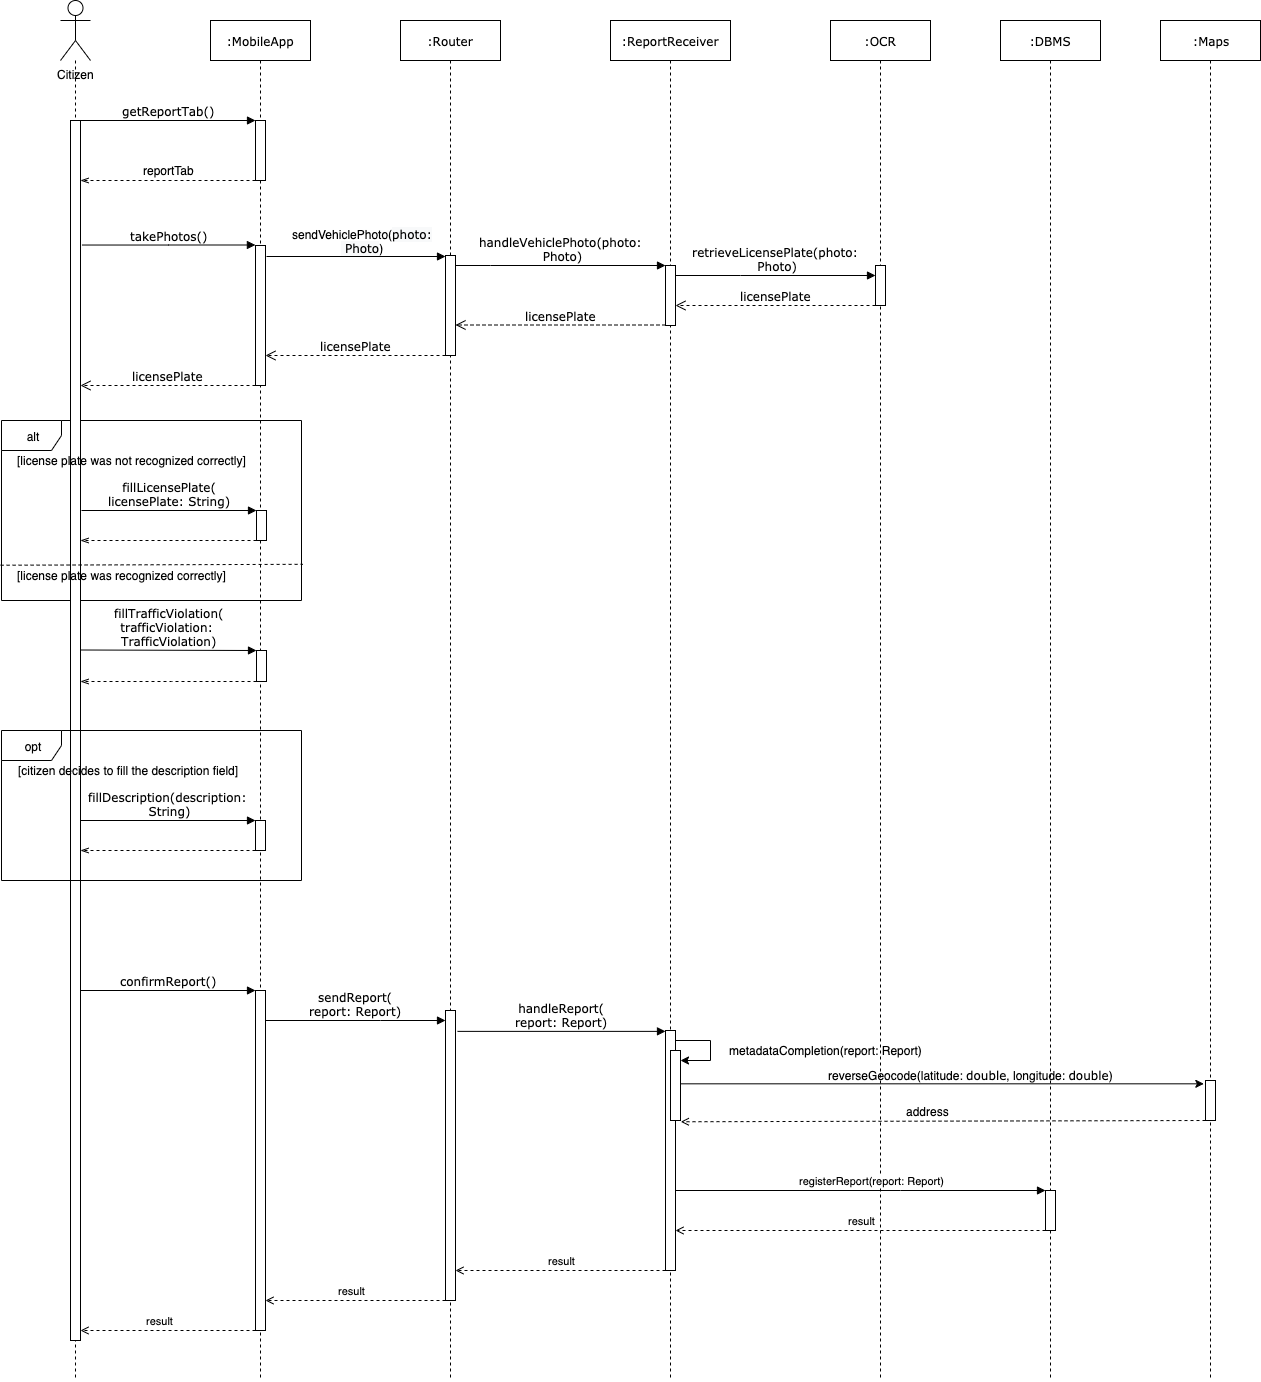
\includegraphics[width=\linewidth]{Images/SequenceDiagramReportViolation}
	\caption{Report a violation sequence diagram.}
\end{figure}
In this sequence diagram the use case in which a citizen reports a traffic violation is shown. After detecting a violation in the streets, the citizen selects the report tab from the main tab of the SafeStreets mobile app. In this case, the report tab has no information to retrieve from the SafeStreets server, which is the case of other services, so the app opens the tab immediately. At this point, the citizen uses the app's internal photo camera service to take photos of the violation, making sure that the first photo contains the transgressor's vehicle with its license plate. After the citizen has completed this first part of the report, the app sends the first photo to the 'Router' component, which forwards it to the 'ReportReceiverManager'. This component uses the external OCR service to recognize the license plate of the vehicle from the photo it received. Then 'ReportReceiverManager' returns the license plate to the 'Router', and this sends the license plate back to the mobile app that updates the license plate field. At this point the citizen checks whether the license plate was recognized correctly, if not he inserts it manually. Then he chooses the traffic violation type, and he optionally fills the description field. The citizen confirms the report, and the mobile app sends the report with GPS coordinate to Router, which forwards it to 'ReportReceiverManager'. This component completes the report with metadata such as timestamp, GPS coordinates and address retrieved from the coordinates, userID, and a 'pending' status. Finally, it registers the report in the system's database.

\subsection{Analyze aggregate data}
\begin{figure}[H]
	\centering
	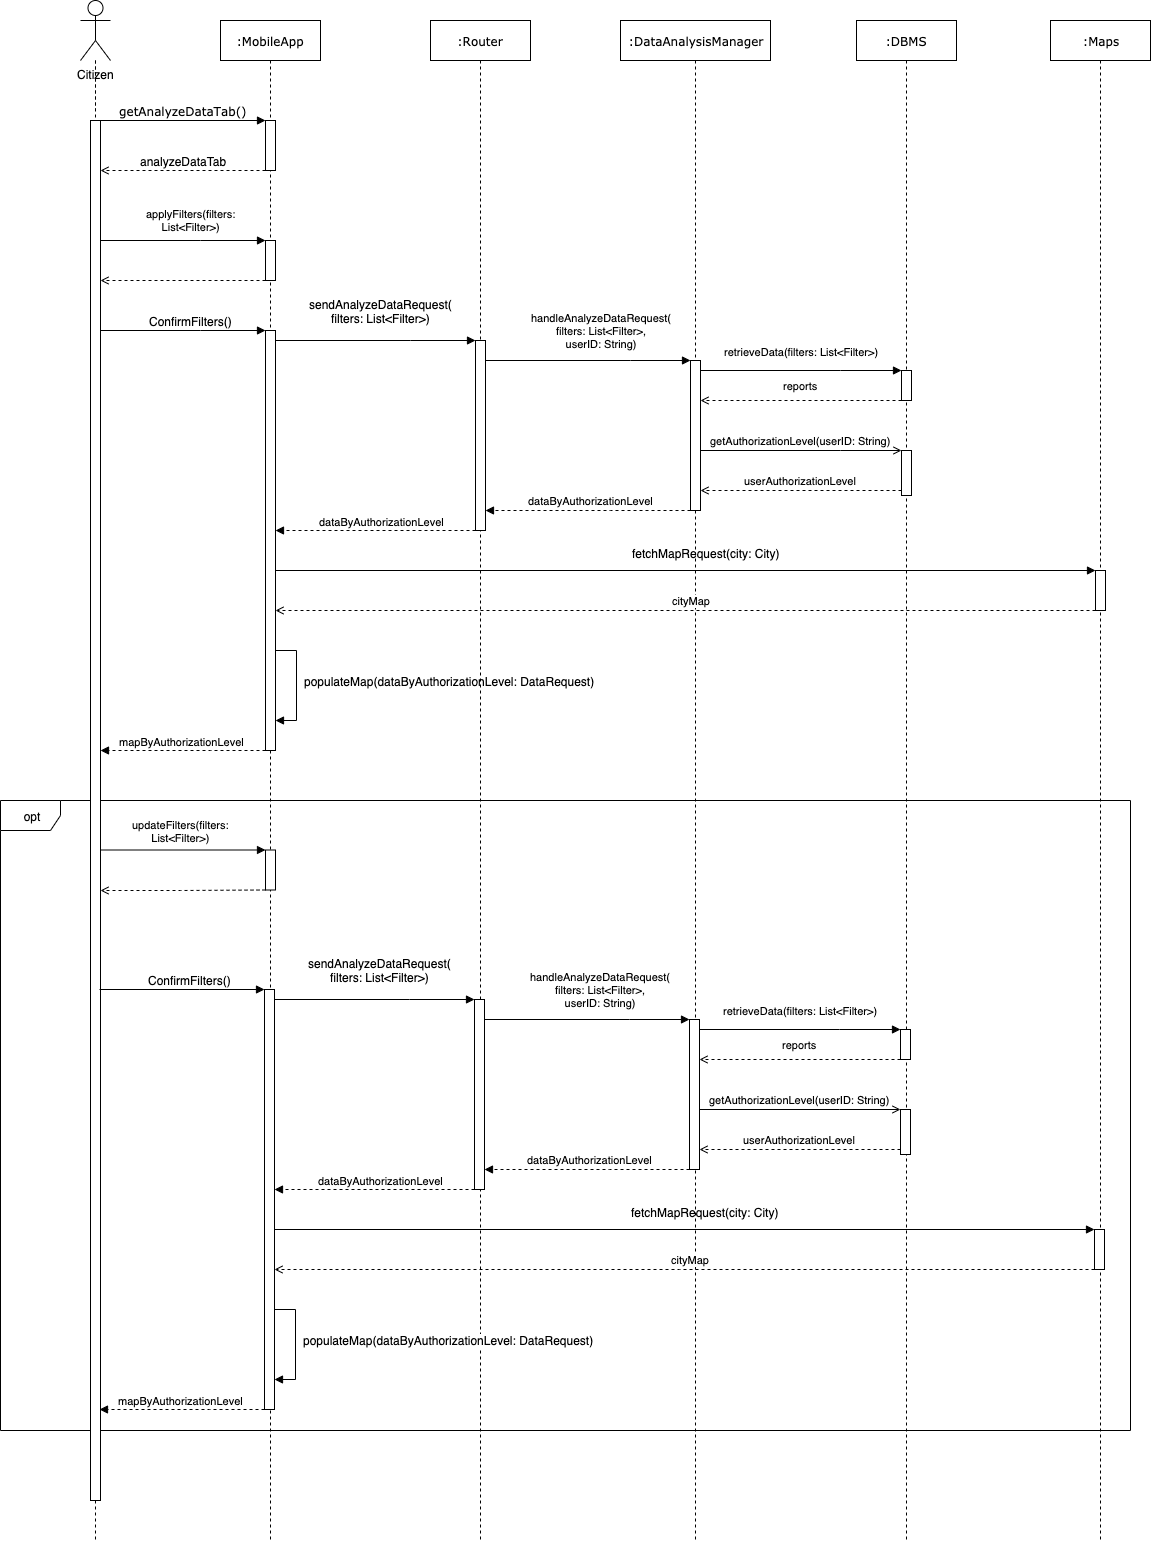
\includegraphics[width=0.95\linewidth]{Images/SequenceDiagramAnalyzeAggregateData}
	\caption{Analyze aggregate data sequence diagram.}
\end{figure}
In this sequence diagram the use case in which a citizen wants to analyze aggregate data is presented. First of all, the citizen selects the analyze aggregate tab from the mobile app main tab. In this tab the citizen selects the filters that are useful for his analysis; examples of filters are the timestamp interval, the location 	and type of the violation. After the citizen has confirmed the filters for his analysis, the mobile app sends an analyze data request with the filters to 'Router'. This component forwards the request to 'DataAnalysisManager', which retrieves data according to the filters from the system's database. Then 'DataAnalysisManager' retrieves the authorization level of the citizen from the database using the userID retrieved from the session and sends back to 'Router' appropriate data according to the authorization level of the user. If the user is a citizen, like in this case, license plate, report submitter info and supervisor info are not sent back to the client, whereas if the user is an authority, all data of the reports are sent back so that the authorities can check the data more accurately, e.g. check the license plate of the most frequent transgressor. At this point, 'Router' forwards the data back to the mobile app, that fetches the map of the city the citizen is interested in and populates the map for visualization. After visualizing the map, the user can update the filters whenever he wants to, and the retrieval of the new map with the new filters is the same as in the above description for the first retrieval of the map. The update of the filters can be done zero or more times depending on the user's preference.

\subsection{Violation validation}
\begin{figure}[H]
	\centering
	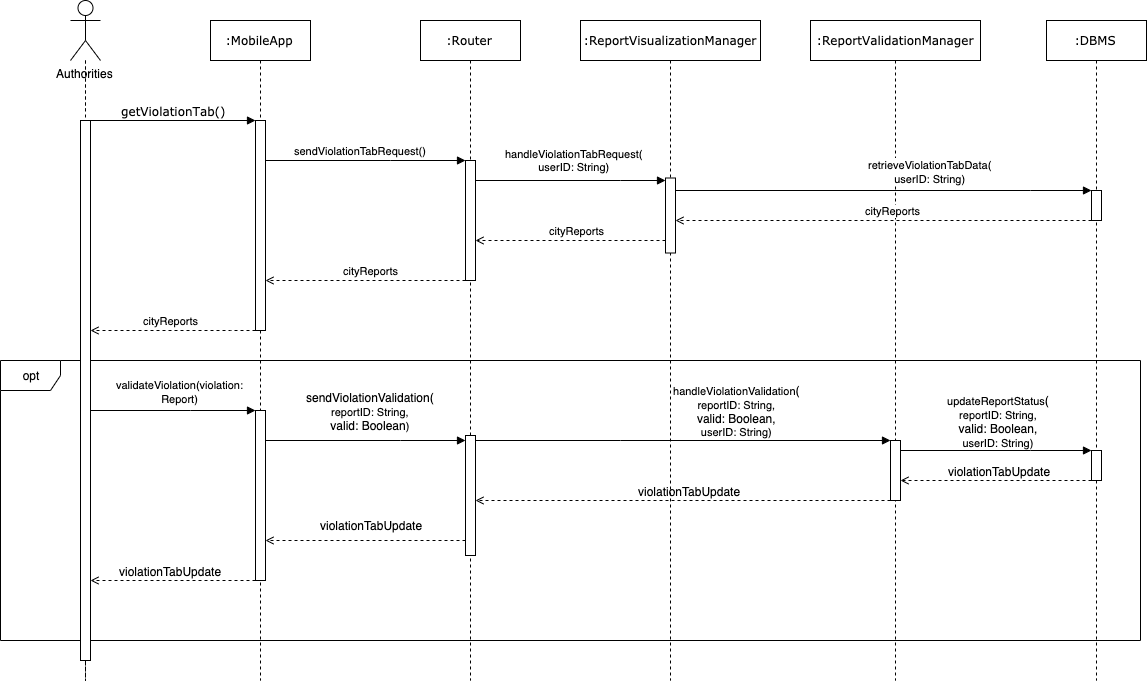
\includegraphics[width=\linewidth]{Images/SequenceDiagramViolationValidation}
	\caption{Violation validation sequence diagram.}
\end{figure}
In this sequence diagram the use case in which an authority validates a violation report is shown. After the authority has selected the violation tab, the mobile app sends a request to retrieve data for the violation tab to 'Router', which forwards the request to the 'ReportVisualizationManager' component. This component verifies that the client that requested the violation tab is an authority (this passage is not shown in the diagram for simplicity, anyway in this case the actor sending the request is an authority, so the system continue with the process) and after that it retrieves the reports related to the city in the jurisdiction of the requesting authority, and finally sends back the reports of that city back to 'Router', which forwards it back to the mobile app. Now the authority can visualize and select a report to validate, and this part can be done zero or more times depending on the number of reports to be verified. After validating/invalidating a report, the mobile app sends a violation validation message with the reportID and the validity of the report to 'Router', which forwards it to 'ReportValidationManager'. The last component updates the status of the report, by changing the 'pending' status to 'validated'/'invalidated' and adding the authority's userID to the supervisor field in the database, and returns the updated report as a violation tab update message to 'Router' (the diagram above assumes the success of the operation). Finally, 'Router' forwards the message back to the mobile app, which updates the changed report for visualization.

\subsection{Suggestion evaluation}
\begin{figure}[H]
	\centering
	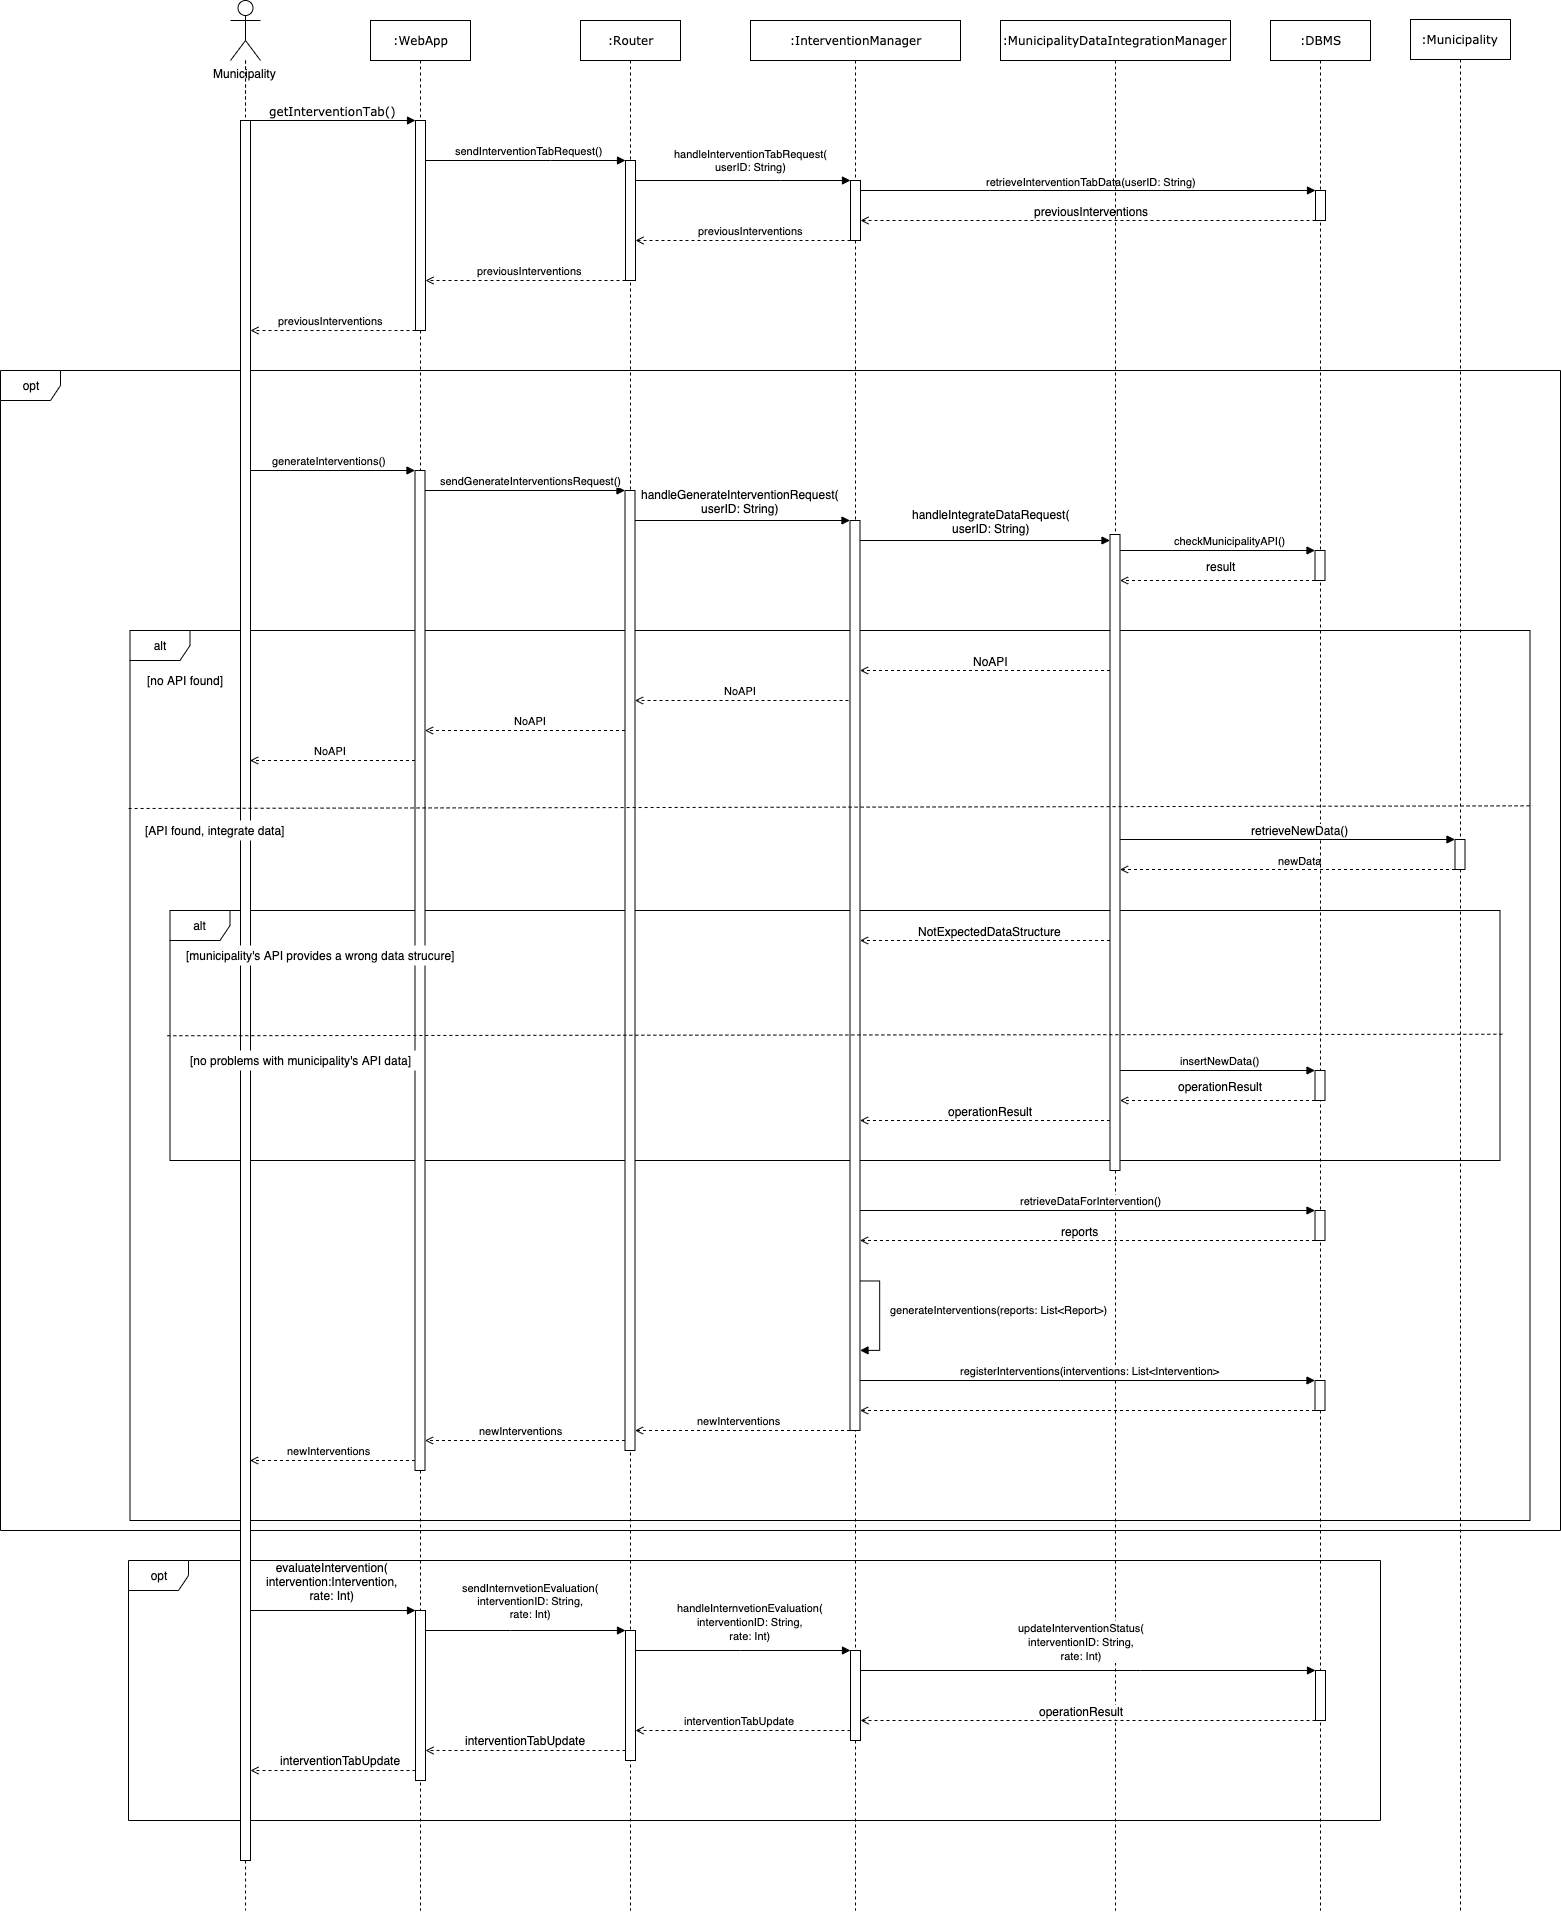
\includegraphics[width=\linewidth]{Images/SequenceDiagramSuggestionEvaluation}
	\caption{Suggestion evaluation sequence diagram.}
\end{figure}
In this sequence diagram the use case in which a municipality generates and evaluates the interventions is shown. After the municipality has selected the intervention tab, the webapp of SafeStreets sends an intervention tab request to 'Router'. Then 'Router' forwards the request to the 'InterventionManager', which retrieves the previously generated interventions from the system's database after checking from session who the user is (so that can retrieve the municipality's city) and sends back to the webapp through the 'Router' component. At this point, the municipality can decide whether to generate new reports or not. If it decides not to generate new interventions, it can just visualize the previously generated internvetions, if any present, or even evaluate them. Whereas if the municipality decides to generate new interventions, the system sends a generate intervention request to 'Router', which forwards it to 'InterventionManager'. This component sends an integrate data request to 'MunicipalityDataIntegrationManager' to check whether the municipality provided an API or not. If no API is present then this data integration process is aborted, otherwise it tries to retrieve new data from the municipality. If the data provided by the municipality does not conform with SafeStreets API an error is generated, and 'InterventionManager' proceeds to generate interventions without any data integration, otherwise the new data is inserted into SafeStreets' database. Finally, 'InterventionMangaer' retrieves all relevant data from the database and generates a possible list of interventions that is stored in the database and sent back to the client via 'Router'. Now the municipality can inspect the newly generated interventions and decide whether to rate them or not. If it decides to rate them, it needs to give a score (e.g. between 0 and 5) as a measure of the quality of the suggestions. The score with the ID of the intervention is sent to 'Router', which forwards it to 'InterventionManager' to update the database with the new information. An update is then sent back to the client to keep the data between the client and the server synchronized.	